\documentclass[../main.tex]{subfiles}

\begin{document}
\section{Problem Definition} \label{sec:prob_def}
We study the pursuit-evasion problem in indoor environments where $k$ pursuers search one evader. The goal of the pursuers is to hold the evader physically in close proximity.
%We study the problem of multiple pursuers and one evader in an indoor environment. 
%Our problem is based on indoor pursuit evasion scenario with a
The configuration of the environment is known to the pursuers but not necessarily known to the evader. We assume a static environment and discretize the environment into a grid world. For each time stamp, both a robot (pursuer) and a target (evader) can move to an adjacent cell on the grid map, or choose to stay in the same cell, which means they have the same base action space in the grid world. We assume the line-of-sight model of the robotic pursuers, which means the robots are able to see the target if there is no obstacle or wall blocking the sight, otherwise they do not directly know
%have no information of 
the target location.

Let the state of the $i$th robot $R_i$, $i = 1, 2, \cdots, k$, at time $t$ be $s_{R_i}(t)$ and the state of the target $T$ at time $t$ be $s_T(t)$. We assume a 4-connected grid so the action space of both robot and target is $A = \{N, E, W, S, Z \}$,
%\remove{\ks{since you are using R for the robot, please use Z for the no-op to avoid confusion}}
which corresponds to move to North, East, West, South, and remain in the current cell (i.e., no-op). The transition by applying an action to a given state of a pursuer is deterministic, which indicates the probability of arriving the next state ${s^\prime_{R_i}}$ from the current state $s_{R_i}$ is $p({s^\prime_{R_i}}, a, {s_{R_i}}) = 1$. Consider $A_v \subseteq A$ to be a valid set of actions for a given state which satisfies each action $a \in A_v$ and does not lead to collision to environment obstacles or walls. In our current scenario, we assume the target moves randomly with a uniform distribution over its action space. Therefore, we have the probability of action $a$ at a given state $s$:
\begin{equation}
p(a) = \begin{cases}
    \frac{1}{|A_v|}, & a \in A_v \\
    0, & a \not \in A_v.
    \end{cases}
\end{equation}
The transition state is defined as one where a pursuer catches the evader, which means that the pursuer and the evader are in the same grid cell at the same time, i.e., $s_{R_i}(t) = s_T(t)$. 

The objective of the pursuers is to find an optimal policy $\pi^\star$ that minimizes the expected time of capturing the evader. Since the reward is discounted, the goal is equivalent to maximizing the expected reward for the pursuers, which is: 
\begin{equation}
\pi^\star = \text{arg} \max_{\pi}{V(s)}. 
\end{equation}

%\cn{(Comment: No equation describing the objective mathematically?)}

\section{Hybrid Hierarchical POMDP} \label{sec:HHPOMDP}
In this section, we review a standard Multi-agent POMDP with a direct joint state space. Then we introduce our method of modeling the environment with convex hulls and borders. We also describe our HHPOMDP structure in detail and define the transition and reward functions accordingly.

\subsection{Multi-agent POMDP} \label{sec:MPOMDP}
A \textit{Partially Observable Markov Decision Process} (POMDP) describes a stochastic process
%with states 
where some of the state variables may not be directly observable~\cite{hauskrecht2000value}.
%that are partially observable.
The process is described by $(S, A, \Theta, T, O, R, \gamma)$, where $S$ is the state space, $A$ is the action set, $\Theta$ is the observation set, $T:S \times A \times S$ is the transition matrix given states, actions, and the next states, $O: S \times A \times \Theta$ is the probability of observations given states, actions and the observation tuple, $R: S \times A \times S$ is the reward given states and action transitions, and $\gamma$ is the discount factor. The goal is to compute an optimal policy $\pi^\star: S \times O \rightarrow A$ that maps from each state and observation pair to an action that maximize the expected discounted reward. 

For multi-agent POMDP with $k$ agents \cite{pynadath2002communicative}, each state $S = S_1 \times S_2 \times \cdots \times S_k$, action set $A = A_1 \times A_2 \times \cdots \times A_k$, observation set $O = O_1 \times O_2 \times \cdots \times O_k$ are all joint state space of each agent. Similar with single agent POMDP, the multi-agent POMDP tries to compute an optimal joint policy $\pi^\star: (\pi_1^\star, \pi_2^\star, \cdots, \pi_k^\star)$ that each $\pi_i^\star: S_i \times O_i \rightarrow A_i$ maps from each state and observation pairs to a corresponding action that maximize the expected discounted reward.

\subsection{Modeling of Environments using Convex Hulls} \label{sec:env_model}
%To utilize the indoor environment characteristics, we discretize the world map configuration into convex hulls on top of the grid world. 
We convert the grid map of an indoor environment into a set of convex hulls. This representation of the environment reduces the size of the state space to a great extent but does not lose necessary information regarding the environment. By definition of convex hull, it is guaranteed that the target is within the sight of a pursuer.
% \smallskip

% \noindent \textbf{Proposition 1.} A target $T$ inside a convex hull can be directly observed by a pursuer $R_i$ located in the same convex hull.
% \smallskip

% \noindent \textbf{Proof.} A convex hull of a set of points $C$ in a Euclidean space is defined as the smallest convex set that contains $C$ where any line segment joining any two points in $C$ is also inside the set. Since the locations of $T$ and $R_i$ are in $C$, they can be connected by a line segment, which indicates that $T$ is in the line of sight of $R_i$.
% \qed

With this abstraction of the environment, grid cells could be separated and grouped into regions, thus we could utilize the environment characteristics for planning and reduce the state space.
%to a great extent.  
%\ks{You need more motivation and discussion about the usefulness of the convex hull.} \ys{I've added some. Not sure if good enough.}

\begin{figure}
    \centering
    \begin{subfigure}[b]{0.3\textwidth}
        \centering
        \frame{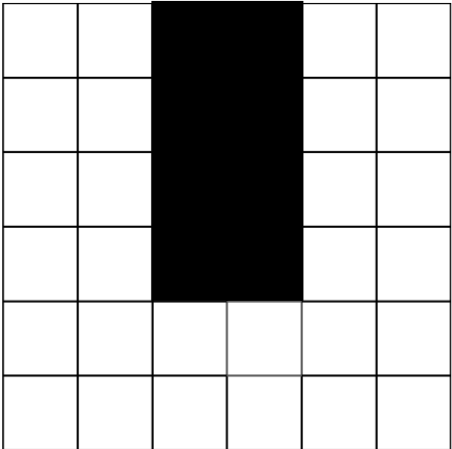
\includegraphics[height=3cm]{grid_world.png}}
        \caption{Grid Map}
        \label{fig:grid_map}
    \end{subfigure}
    \begin{subfigure}[b]{0.3\textwidth}
        \centering
        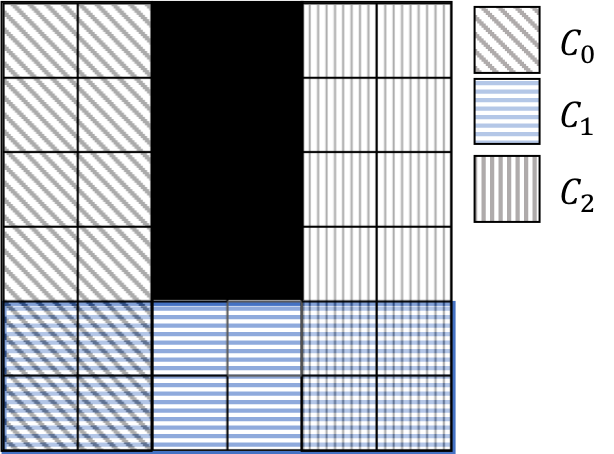
\includegraphics[height=3cm]{grid_convex.png}
        \caption{Convex Hull}
        \label{fig:convex_hull}
    \end{subfigure}
    \begin{subfigure}[b]{0.3\textwidth}
        \centering
        \frame{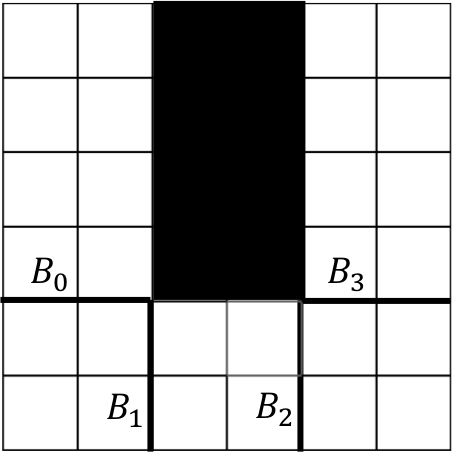
\includegraphics[height=3cm]{grid_border.png}}
        \caption{Convex Hull Borders}
        \label{fig:convex_hull_border}
    \end{subfigure}
    \caption {Modeling the grid world. (a) The world map is discretized into grids. (b) Overlapping convex hulls are defined based on the free space in the map. (c) The intersections of convex hulls form borders.} 
    \label{fig:map_discrete}
      
\end{figure}

As shown in Fig.~\ref{fig:map_discrete}, the grip map of the environment is modeled in the following way:
%\ks{is this the only map you use? It is very simple.} \ys{I have many more maps in the result part}
%In Fig.~\ref{fig:grid_map}, there are walls and obstacles in the original environment map. The black grid cells are walls and the white area is the free space.
%We model the environment with convex hulls and each convex hull expands to its maximum coverage area.
Fig.~\ref{fig:grid_map} shows the original environment map in grids where the black grid cells represent walls and obstacles and the white area represents the free space. We model the environment by grouping grid cells into convex hulls such that the number of convex hulls is minimized.
A convex hull is denoted as $C_i$, which also will be used as a state variable in the state space of the evader. As shown in Fig.~\ref{fig:convex_hull}, the convex hulls may have overlapping areas. The overlapping areas of the adjacent convex hulls form borders shown in Fig.~\ref{fig:convex_hull_border}. A border is denoted as $B_i$, which will be used as a state variable of the state space of the pursuers. At each convex hull border $B_i$, a pursuer is able to directly observe the target in any of the adjacent convex hulls as proved in Proposition 1.
%\ks{You need to describe the figure in detail.  Where are the walls and how are thy notated? The only thing we see is a big black area. Is this the obstacle, a wall or what? To which convex hulls doe the unlabelled areas of (b) belong to? To all of them? Then you need to say this. What is the role of borders? How are they defined formally?} \ys{modified accordingly}
%\cn{(Comment: you need to make clear whether you developed an algorithm that models the environment using convex hulls or you manually did it. I know you did the latter. So you may have to discuss about how the modeling process can be automated.)} 
In this present work, the convex hulls are generated through unautomated processes. However, it can be generated directly from the input map if we iterate through all the cells and use any standard convex hull finding algorithm, for example Jarvis’s Algorithm~\cite{eddy1977new}.

\subsection{Hybrid Hierarchical POMDP Structure} \label{sec:hhpomdp_struct}
For multi-agent planning, the direct way for the optimal result is to plan on the joint state space of all robots as described in Sec.~\ref{sec:MPOMDP}. However, the complexity grows exponentially with the number of robots. For multi-agent POMDP, the complexity is much higher than direct joint MDP since it is necessary to track history and record the belief space vector. Note that the complexity of POMDPs even with a single agent is PSPACE-complete~\cite{papadimitriou1987complexity}.

We notice that when the target is not observable to any of the pursuers, its exact position on the grid map does not make a significant difference to the exploration plan of the pursuers because the pursuer needs to ``see" the target (i.e., both parties are in the same convex hull) before catching. Instead, only the convex hull in which the target lies within influences the next location of pursuers. 
%In this case, 
Thus, the state space which is partially observable to the pursuers could consist of
%be the abstract 
the convex hull borders while the exact location of the target on the grid cells is omitted. 
%However, 
On the other hand, when the target and pursuers are in the same convex hull, the location of the target is fully observable to the pursuers. Thus, it is not necessary to keep track of any observation history, which means that an MDP can be used to improve computational efficiency. Therefore, we propose a \textit{Hybrid Hierarchical structure} of MDPs and POMDPs as shown in Fig.~\ref{fig:pomdp_struct}.

%\ks{You need to define formally what the hybrid model is. You need to justify whay you are breaking up the model in the way you do. why have MDPs and POMDPs? Are there going to be consistency problems as one goes between levels? etc etc.} \ys{added more initiatives and description above}

\begin{figure}
    \centering
    \includegraphics[width=0.89\textwidth]{hierachy.png}
    \caption{The Hybrid Hierarchical POMDP Structure. The structure consists of the base MDPs for the cases where the evader is visible to the pursuers, the abstract POMDPs for the evader states that are not directly observable, and the transition states bridging between the base MDPs and abstract POMDPs.}
    \label{fig:pomdp_struct} 
\end{figure}

%\ks{please explain the figure in detail.} \ys{more description added in the next paragraph.}
%\cn{(Comment: you used $n$ for the number of robots in the problem definition. So make the notation consistent.)} \ys{(all changed to k)}
Specifically, consider $k$ pursuers (robots) and one evader in a grid world environment discretized into $N$ convex hulls and $M$ convex hull borders. We denote the location of the evader (target) with a belief space vector $b = [b_0, b_1, \cdots, b_{N-1}]$. As shown in Fig.~\ref{fig:pomdp_struct}, the nodes on top shows the abstract POMDP nodes, which is the joint state space of all pursuers. The nodes in the middle is transition states where all the belief vector of target location results in a specific convex hull. The nodes in the bottom are the base MDP nodes contains only the location of one pursuer and the target in the grid world. Let the state of robot $j$ be $S_{R_j}$ and the state of target to be $S_T$, the states in the abstract POMDP level is denoted as $S^p_i$, transition states as $S^t_i$, and the base MDP states are $S^b_i$. 
%\cn{(Comment: you need to begin with how the structure is constructed. Readers have no idea of the abstract POMDP \ys{level}, transition states, and the base MDP states yet.)} \ys{(Modified above. More details in the paragraph below.)}

The hybrid POMDP tree has a height of three. Level 1 is the joint abstract POMDP of all the pursuers' and target's state spaces $S^p_i: S^p_{R_1} \times \cdots \times S^p_{R_k} \times S^p_{T}$, where the target state space is the Cartesian product of belief of each individual states $S^p_T = \prod_{i =0}^{k-1} B_i$. Each robot has a starting state, the POMDP policy tree grows by applying all valid actions and observations $(a, o)$, and the belief space vector is updated accordingly.
The belief space vector is maintained with a mixed observability since we assume all robots are connected, the locations of all pursuers are known by all robots, and only the target location is partially observable.
Level 2 is the transition state when the belief space shrinks to one convex hull, and the target is visible to one of the robots.
Level 3 is the base MDP of the joint space of one robot $R_j$ and the target $T$, $S^b_i = S^b_{R_j} \times S^b_T$. When the target goes out of the line of sight of $R_j$, the state of the robot returns to Level 2 and if the belief space expands, it may return to Level 1. 

\subsection{Transitions and Rewards} \label{sec:trans_reward}

%\ks{Fix the notation. Also, you need to use citations where appropriate. You are basing your work and notations on the work of others, so you need to cite. Also here you need to justify your assertions.} \ys{citeation added}


\subsubsection{Base MDP}
The base MDP is fully observable and follows the standard Bellman equation for dynamic programming~\cite{bellman2013dynamic}: 
\begin{equation}
    V^{*}(s^b) = \max_{a^b \in A^{b}} \sum_{{s^{b}}'} T^b(s^b, a^b, {s^{b}}') [R(s^b, a^b, {s^{b}}') + \gamma V^{*}({s^{b}}')] 
\end{equation}%
where $s^b$ is the current base state in the grid world, which is the coordinate on the grid map, $\gamma$ is the discount factor, ${s^b}'$ is the neighboring states of state $s^b$, and $T^b$ is the transition matrix and $A^b$ is the action space for the base MDP, which is the same as the action space in Sec.~\ref{sec:prob_def} that is $A^b = \{N, E, W, S, Z \}$. 

Each base MDP state is the joint space of the target and the robot in the same convex hull $s^b = s_R^b \times s_T^b$. The action spaces of the robot and target are the same, which form the joint action space for the base MDP $A^b = a_R^b \times a_T^b$. Since the target moves randomly, the robot has a deterministic outcome for applying a given action,
%\cn{(Comment: did you describe this assumption of deterministic state transitions in the problem formulation?)} \ys{(added in the problem formulation part)}, 
and the transitions of the robot and target are independent
%\cn{(Comment: deterministic transitions have nothing to do with the independence of transitions of the robot and the target? if a transition is probabilistic, does it affect the independence? Aren't they still probabilistic?)} 
the transition probability is uniformly distributed over the all valid target neighboring states $S_T^b$: 
\begin{equation}
\begin{aligned}
    T^b(s^b, a^b, {s^b}') = p({s^b}' | s^b, a^b)
    &= \frac{1}{|S_T^b|}.
\end{aligned}
\end{equation}
For the next state ${s^b}'$, it is possible that the target might disappear from sight. If this happens, the next state will go back to the transition state and might also further go back to the abstract POMDP level if the belief space vector changes. This procedure is described in Alg.~\ref{alg:expand_base}.

Reward is only given to the final terminal state when one of the robot catches the target, which is when the target and a robot is in the same cell on the grid map: 
\begin{equation}
R(s^b, a^b, {s^b} ') =
    \begin{cases}
    r, \ \exists j \in [0, k)\ s.t.\ s_{R_j}^b=s_T^b \\
    0, \ \text{otherwise.}
    \end{cases}
\end{equation}


\begin{algorithm}[H]
    \caption{Expand Base Node}
    \label{alg:expand_base}
    \begin{algorithmic}[1]
    \Input{$c$: current node to be expanded, $A$: action set}
    \Output{node set to be expanded}
    \Function{ExpandBase}{$c$, $A$} 
    \For {$a$ in $A$}
        \State $n$ $\gets$ getNeighborNode($c$, $a$)
        \If {not isVisible($c$.robot, $c$.target)}
            \State $n$.type $\gets$ transition
        \Else{}
            \State $n$.type $\gets$ Base
        \EndIf
        \State $c$.childList.append($n$)
    \EndFor
    \Return{$expandSet$ $\cup$ $c$.childList}
    \EndFunction
    \end{algorithmic}
\end{algorithm}
\begin{algorithm}[H]
\caption{Expand Transition Node}
\label{alg:expand_term}
\begin{algorithmic}[1]
\Input{$c$: current node to be expanded}
\Output{node set to be expanded}
\Function{ExpandTransition}{$c$}
\If {not isVisible($c$.robot, $c$.target)}
    \State $n$ $\gets$ Node($c$)
    \State $n$.type $\gets$ POMDP
    \State $c$.childList.append($n$)
\Else {}
    \State $baseList$ $\gets$ getBaseGrid($c$.belief)
    \For {$b$ in $baseList$}
        \State $n$ $\gets$ Node($b$)
        \State $n$.type $\gets$ Base
        \State $c$.childList.append($n$)
    \EndFor
\EndIf
\Return{$expandSet$ $\cup$ $c$.childList}
\EndFunction
\end{algorithmic}
\end{algorithm}

\begin{algorithm}[H]
\caption{Expand POMDP Node}
\label{alg:expand_pomdp}
\begin{algorithmic}[1]
\Input{$c$: current node to be expanded, $\Theta$: observation set, $A$: action set}
\Output{node set to be expanded}
\Function{ExpandPOMDP}{$c$, $\Theta$, $A$} 
    \For {($a$, $o$) in ($\Theta$, $A$)}
    \State $n$ $\gets$ getNeighborNode($c$, $a$, $o$)
    \State $n$.updateBelief()
    \If {max($n$.belief) is 1}
        \State $n$.type $\gets$ transition
    \Else {}
        \State $n$.type $\gets$ POMDP
    \EndIf
    \State $c$.childList.append($n$)
    \EndFor
    \Return{$expandSet$ $\cup$ $c$.childList}
\EndFunction
\end{algorithmic}
\end{algorithm}

\subsubsection{Transition State}
A transition state represents a transition between the abstract POMDP and the base MDP.
%\cn{(Comment: the name is confusing. Transition states would be more intuitive? Terminal means the end of some processes so it sounds like the end of the mission.)}. \ys{(changed to transition)} 
The transition states could be entered from either the base MDP or the abstract POMDP. When the belief space vector shrinks to one cell, i.e, $\exists b_i = 1$, and the target is visible to one of the robot, then the expansion process enters the transition states from the abstract POMDP. The expansion can also come from the base MDP when the target moves away from the line of sight of any robot, and in this case, the system needs to return to the abstract POMDP via those transition states. This procedure is described in detail in Alg.~\ref{alg:expand_term}.'



\subsubsection{Abstract POMDP}
The abstract POMDP has a mixed observability of the state space. The state space is the joint state space of all robot locations (convex hull borders) and the target location (convex hulls).
For robot $R_j$, the state in the abstract POMDP level $s_{R_j}^p$
%\cn{(Comment: again, what is the definition of the ``layer''? layer=level?)} 
includes the convex hull borders which are fully observable. This belief space vector is updated during the expansion of the policy tree (Alg.~\ref{alg:expand_pomdp}) and will enter the transition state if one of the convex hull belief is one. For target $T$, the state space $s_T^p$ is the belief across convex hulls $b = [b_0, b_1, \cdots, b_{N-1}]$ which are partially observable. This formulation gives the mixed observability of state variables and is used to simplify computation in the transition and reward functions.

The state value update follows the traditional Bellman updates, but with the belief space vector~\cite{hauskrecht2000value}
\begin{equation}
    V^* ( b ) = \max _ { a \in A } \left\{ \sum _ { s \in S } R ( s ,a ) b ( s ) + \gamma \sum _ { o \in \Theta } \sum _ { s \in S } T ( o | s ,a ) b ( s ) V^* ( \tau ( b ,o ,a ) ) \right\}
\end{equation}
where $R(s, a)$ is the reward function for action $a$ at a given state $s$, $T ( o | s ,a )$ is the transition probability of having observation $o$ given state $s$ and action $a$. The function $\tau$ represents the information state of the joint space of belief vector $b$, observation $o$ and action $a$.
For our specific problem, the reward of the system only comes from the base MDP in the absorbing state where the target and a robot are in the same cell. Thus, there is no reward in the updates from the abstract POMDP level itself. 

Along with the mixed observability described above, we could simplify the value update based on the full observable states of the robots and only keep track of the belief vector over the target state space. The action space for the abstract POMDP is the joint action of all robots and target, which is the Cartesian product $A = A_T^p \times \Pi_{j}A_{R_j}^p$. Similarly, the robot state space is also the Cartesian product $s_R^p = \Pi_{j}s_{R_j}^p$. Since the robot transitions are deterministic and independent from each other as well as the target, the transition probability is only dependent on the target transitions, which is uniformly distributed over its adjacent convex hulls that the robot can move, and robots' visibility. Thus, the transition probability is
\begin{equation}
T(o | s,a) = T(o| {s_T ^p}', {s_R ^p}') \cdot T({s_T ^p} ' | s_T ^p) \cdot T({s_R ^p} ' | s_R ^p). 
\end{equation}
Then we have the following modified Bellman equation:
\begin{equation}
\displaystyle
V^* ( s^p ) = \max _ { a \in A } \left\{ \gamma \sum_{ o \in \Theta } \sum_{ {s^p_T} '} \sum_{ {s^p_R} ' } T ( o | {s_T^p}' , {s_R^p}') T({s_T^p} ' | s_T^p) T({s_R^p} ' | s_R^p) b ( s_T^p ) V ( \tau ( b ,o ,a ) ) \right\}.
\end{equation}

The HHPOMDP system is solved by value iteration based on forward exploration from the root state \cite{hauskrecht2000value}, which will only search in all reachable belief states instead of the full span of belief vectors.

%\cn{(Comment: the following algorithms should be called out in the main text.)}



\section{Experiment Results} \label{sec:result}
We implemented the HHPOMDP algorithm in Python and built a simulation environment on grids in Robot Operating System (ROS). The program is running on Intel Xeon CPU of 2.30GHz with Ubuntu 16.04.4 LTS. %\cn{(Comment: since you are mentioning about the computation time below when you talk about the standard POMDP, you need to describe the machine setup--CPU, RAM, and OS--to give an idea that how 48 hours of running time is comparable to other systems.)} 
The simulation system consists of an environment canvas node for displaying the map, a pursuer planning node, and a random target node. Firstly, we run our simulation based on the following four maps in shown Fig.~\ref{fig:env_map}. These four maps have different indoor structures. Map 2 has a loop and Map 3 has two loops, which would give the target more possibility to evade and hide. In these maps, catching the target is more difficult for the pursuers than those maps with dead-end as the target has more chances to get out from the line of sight of the pursuers.

\begin{figure}
\captionsetup{skip=0pt}
    \centering
    \begin{subfigure}[b]{0.22\textwidth}
        \centering
        \frame{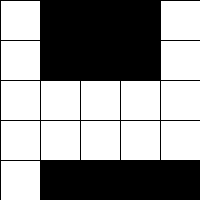
\includegraphics[width=\textwidth]{map1.jpg}}
        \caption{Map 1}
        \label{fig:map1}
    \end{subfigure}\
    \begin{subfigure}[b]{0.22\textwidth}
        \centering
        \frame{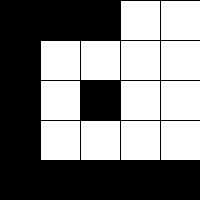
\includegraphics[width=\textwidth]{map2.jpg}}
        \caption{Map 2}
        \label{fig:map2}
    \end{subfigure}\
    \begin{subfigure}[b]{0.22\textwidth}
        \centering
        \frame{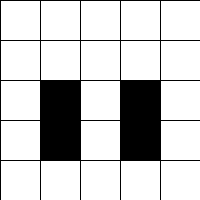
\includegraphics[width=\textwidth]{map3.jpg}}
        \caption{Map 3}
        \label{fig:map3}
    \end{subfigure}\
    \begin{subfigure}[b]{0.22\textwidth}
        \centering
        \frame{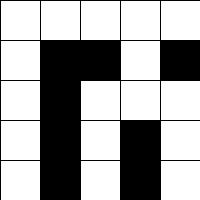
\includegraphics[width=\textwidth]{map4.jpg}}
        \caption{Map 4}
        \label{fig:map4}
    \end{subfigure}
    \caption{Environment maps with different indoor structures}
    \label{fig:env_map}
\end{figure}

Fig.~\ref{fig:node_map123} shows the number of nodes expanded in Map 1--4 with both the HHPOMDP and a standard POMDP. The graph is drawn in a log scale, thus our method significantly decreases the number of nodes expanded. The number of nodes for the standard POMDP method is also exponentially increasing as the number of robots grows. The standard full POMDP is solved using a standard value iteration as described in~\cite{hauskrecht2000value}. Solving the standard POMDP takes more than 48 hours with more than 2 robots in our simulation environment.
%\cn{(Comment: what did you use to solve the standard POMDP? Cite the work.)}


\begin{figure}
\captionsetup{skip=0pt}
    \centering
    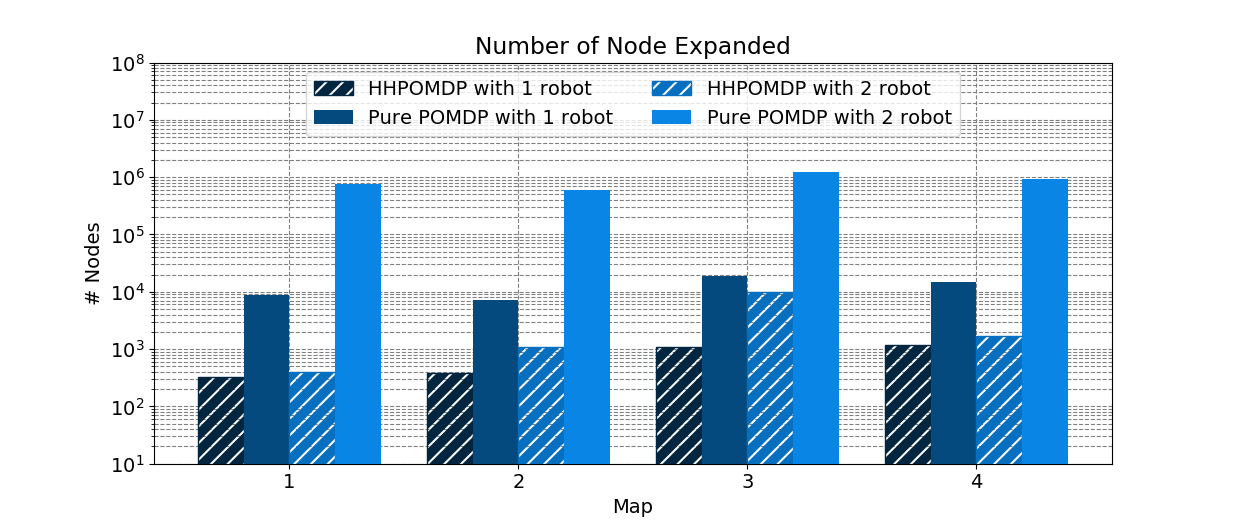
\includegraphics[width=\textwidth]{new_node_map123.png}
    \caption{The number of nodes expanded in our HHPOMDP and a standard POMDP}
    \label{fig:node_map123}
\end{figure}

We run our method in Map 4 with multiple robots up to three. The result is shown in Fig.~\ref{fig:map4robot}.

\begin{figure}
\captionsetup{skip=0pt}
    \centering
    \begin{subfigure}[b]{0.48\textwidth}
        \centering
        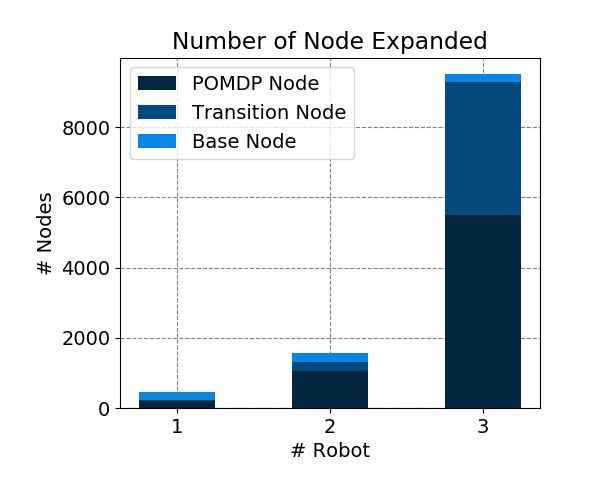
\includegraphics[width=\textwidth]{new_node_map4.png}
        \caption{}
        \label{fig:node_map4}
    \end{subfigure}
    \begin{subfigure}[b]{0.48\textwidth}
        \centering
        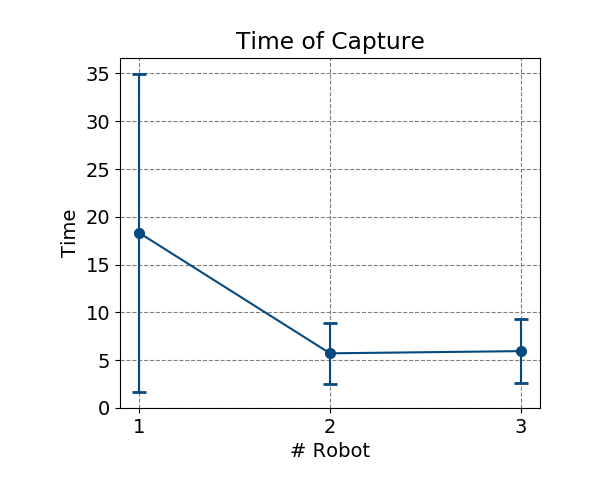
\includegraphics[width=\textwidth]{new_time_map4.png}
        \caption{ }
        \label{fig:time_map4}
    \end{subfigure}
    \caption{Results with Map 4 with different numbers of robots}
    \label{fig:map4robot}
\end{figure}

The number of nodes in base MDP is independent from the number of robots, but the number of nodes grows for both the abstract POMDP and transition states. Fig.~\ref{fig:time_map4} shows the time of capturing the target with different numbers of robots. Both the average and standard deviation of the capture time decreases if the number of robots increases from one to two. It remains the same with three robots, mainly because the map only contains dead-ends but not loops, thus increasing the number of robots does not improve the performance of the robots in capturing the target. 

We also tested our algorithm with different sizes of maps as shown in Fig.~\ref{fig:env_map_size}. They are of 8-by-8, 12-by-12, 16-by-16 grid maps with the same structure, i.e., convex hulls and borders. The result with two robots in the three different map sizes is shown in Fig.~\ref{fig:map456_r2}. Since the environment has the same structure, number of nodes for the abstract POMDP remains the same, only the number of the base MDP increases while the size of the map grows. Both the average and standard deviation for the time of capturing the target increases with the map size, since there is more free spaces for the target to move and thus it is more difficult to catch the target.

\begin{figure}
\captionsetup{skip=0pt}
    \centering
    \begin{subfigure}[b]{0.28\textwidth}
        \centering
        \frame{
\includegraphics[width=\textwidth]{map5.jpg}}
        \caption{Map 5}
        \label{fig:map5}
    \end{subfigure}\
    \begin{subfigure}[b]{0.28\textwidth}
        \centering
        \frame{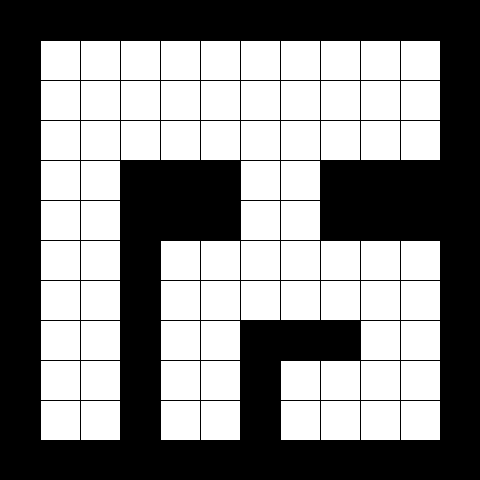
\includegraphics[width=\textwidth]{map6.jpg}}
        \caption{Map 6}
        \label{fig:map6}
    \end{subfigure}\
    \begin{subfigure}[b]{0.28\textwidth}
        \centering
        \frame{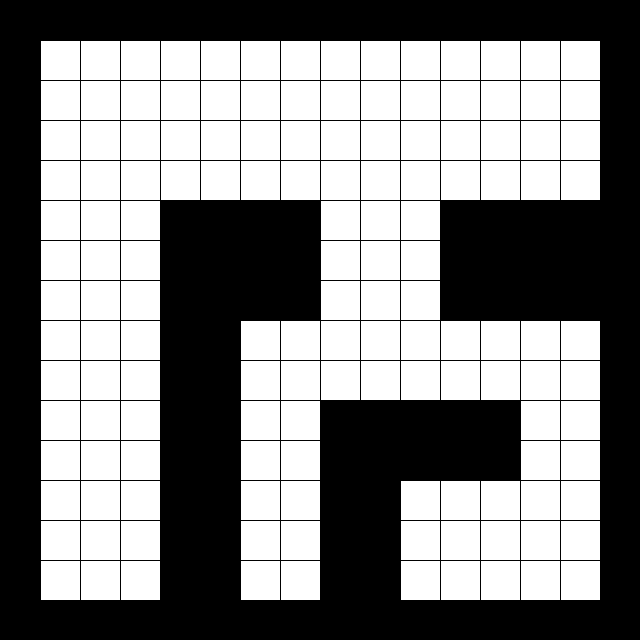
\includegraphics[width=\textwidth]{map7.jpg}}
        \caption{Map 7}
        \label{fig:map7}
    \end{subfigure}
    \caption{Environment maps with different sizes}
    \label{fig:env_map_size}%\vspace{-15pt}
\end{figure}


\begin{figure}%\vspace{-15pt}
\captionsetup{skip=0pt}
    \centering
    \begin{subfigure}[b]{0.48\textwidth}
        \centering
        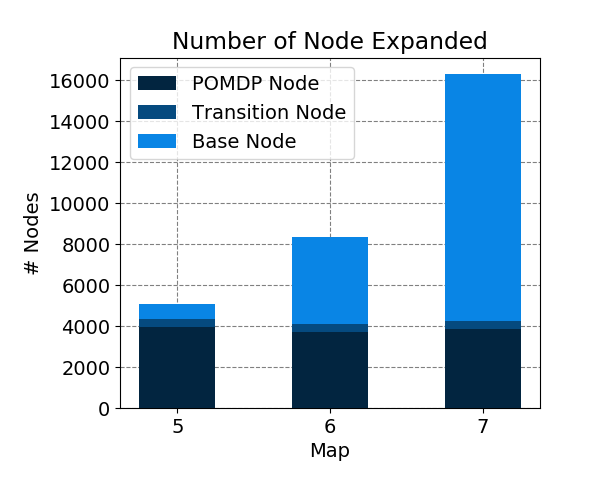
\includegraphics[width=\textwidth]{new_node_map567.png}
        \caption{}
        \label{fig:node_map456}
    \end{subfigure}
    \begin{subfigure}[b]{0.48\textwidth}
        \centering
        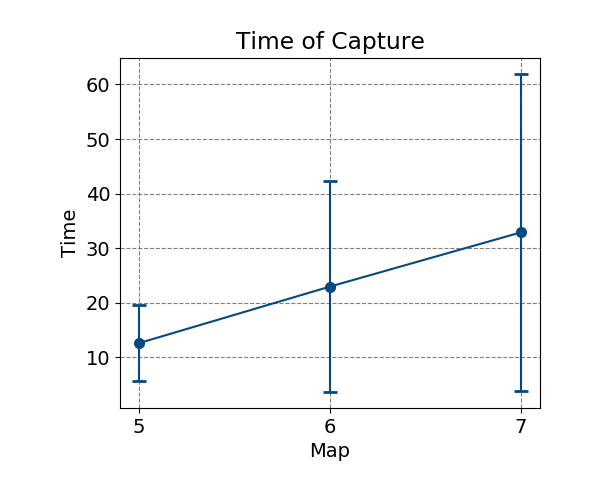
\includegraphics[width=\textwidth]{new_time_map567.png}
        \caption{ }
        \label{fig:time_map456}
    \end{subfigure}
    \caption{Result with 2 robots on maps of different size}
    \label{fig:map456_r2}%\vspace{-25pt}
\end{figure}

\section{Conclusions and Future Work}
This paper presents a scalable algorithm for an indoor pursuit evasion problem using multiple robotic pursuers. We proposed the Hybrid Hierarchical POMDP structure that utilizes the convex hulls of the environment to create abstract states. The algorithm could transit between the base MDP and the abstract POMDP so as to keep track of the target when it disappear during the capture event. We have shown that our algorithm is more scalable than a standard multi-agent POMDP solution and can capture the target within a reasonable time.

The HHPOMDP approach is not limited only to the pursuit-evasion problem discussed in the paper. For other planning problems where an environment abstraction could be made in the lower level, having the hierarchical model would help with reducing computational complexity. The architecture could also be extended to scenarios when the planning tasks could be divided into groups and each group is independent from each other.

Our idea can be extended in the future to consider limited communication. For our current settings, all the robots are fully connected, thus the belief space information is shared across all robots throughout all time stamps. However, in real world applications, keeping all robots connected and exchanging information are both unsafe and limited owing to bandwidth restrictions. Therefore, extension on limited communication, information sharing, and belief space updates will be essential to increase the applicability of this problem. Since our current method is fully centralized, a decentralized version of the algorithm might be needed for the limited communication setting. In addition, we only consider scenarios with one target. However, in many real world scenarios such as search and rescue, there might be multiple moving targets. In this case, task allocation is needed and optimizing over multiple target is challenging in larger state spaces. This would require more abstraction over both the environment and target locations.  

Another limitation of the current structure is that HHPOMDP is solved by the forward exploration in the reachable belief space, which is not efficient with growing state space. A more efficient solver would be needed, possibly with heuristic or sampling in policy trees.
\end{document}